\documentclass[11pt,a4paper]{scrartcl}
\usepackage{color}
\usepackage{ifthen}
\usepackage{ifpdf}
\usepackage[headings]{fullpage}
\usepackage{listings}
\lstset{language=Java,breaklines=true}
\ifpdf \usepackage[pdftex, pdfpagemode={UseOutlines},bookmarks,colorlinks,linkcolor={blue},plainpages=false,pdfpagelabels,citecolor={red},breaklinks=true]{hyperref}
  \usepackage[pdftex]{graphicx}
  \pdfcompresslevel=9
  \DeclareGraphicsRule{*}{mps}{*}{}
\else
  \usepackage[dvips]{graphicx}
\fi

\newcommand{\entityintro}[3]{%
  \hbox to \hsize{%
    \vbox{%
      \hbox to .2in{}%
    }%
    {\bf  #1}%
    \dotfill\pageref{#2}%
  }
  \makebox[\hsize]{%
    \parbox{.4in}{}%
    \parbox[l]{5in}{%
      \vspace{1mm}%
      #3%
      \vspace{1mm}%
    }%
  }%
}
\newcommand{\refdefined}[1]{
\expandafter\ifx\csname r@#1\endcsname\relax
\relax\else
{$($in \ref{#1}, page \pageref{#1}$)$}\fi}
\date{\today}
\chardef\textbackslash=`\\
\usepackage{pdfpages}
\usepackage[utf8]{inputenc}
\usepackage[T1]{fontenc}
\usepackage[german]{babel}
\usepackage{hyperref}
\hypersetup{
	pdftitle={Pflichtenheft},
	bookmarks=true,
}
\usepackage{csquotes}

\usepackage{fancyhdr}%<-------------to control headers and footers
\usepackage[a4paper,margin=1in,footskip=.25in]{geometry}
\fancyhf{}
\fancyfoot[C]{\thepage} %<----to get page number below text
\pagestyle{fancy} %<-------the page style itself

\usepackage{xcolor}
\usepackage{framed}
\definecolor{shadecolor}{RGB}{220,220,220}
\usepackage{float}


\title{Android GO! App - Testbericht}
\author{Gruppe 3}
\date{10.09.17}

% define custom lists
\usepackage{enumitem}
\usepackage{lipsum}

\def\threedigits#1{%
  \ifnum#1<100 0\fi
  \ifnum#1<10 0\fi
  \number#1}

\begin{document}

\begin{titlepage}
	\begin{center}
	{\scshape\LARGE \bfseries Testbericht \par}
	\vspace{1cm}
	{\scshape\Large Praktikum der Softwareentwicklung \\ Sommersemester 2017\par}
	\vspace{1.5cm}
	{\huge\bfseries Android GO! App\par}
	\vspace{2cm}
	{\Large\itshape - Gruppe 3 -\par}
	\vfill
	{\bfseries erstellt von:\par}
	Arsenii Dunaev \\
	Florian Kröger \\
	Tina Maria Strößner \\
	Volodymyr Shpylka \\	
	\vfill
	% Bottom of the page
	{\large 10.09.17 \par}	
	\end{center}
\end{titlepage}

\newpage

\tableofcontents

\newpage
\section{Testszenarien und globale Testfälle des Pflichtenhefts}

\subsection{Weggefallene und geänderte Testfälle}\label{weggefallene Testfälle}
Diverse Testszenarien, die im Pflichtenheft definiert wurde, werde nicht getestet, da sie durch Änderungen im Verlauf der Entwicklung nicht mehr zutreffend sind. Dazu gehören:
\begin{itemize}
	\item[/T0020/] Das Ändern des Benutzeraccounts war ein Wunschkriterium und wurde in der Implementierung nicht umgesetzt.
	
	\item[/T0090/] Hier wurde der Ablauf des Anwendungsfalls während der Implementierung verändert: Anstatt dem Benutzer eine Lliste mit Benutzern mit der passenden E-Mail-Adresse zu zeigen, wird direkt dem Benutzer mit der passenden E-Mail-Adresse eine Gruppenanfrage geschickt. Außerdem können weder Mitglieder noch Administratoren die aktuellen Gruppenanfragen in er App sehen, es werden lediglich vollwertige Gruppenmitglieder in der Gruppendetailansicht angezeigt.
	
	\item[/T0130/]\label{130} Das Hinzufügen von Administratoren ist in der Implementierung nicht umgesetzt. Verlässt ein Administrator die Gruppe, wird diese gelöscht. Der erwartete Reaktion des Testfalls ist die Löschung der Gruppe.
	
	\item[/T0140/] Fällt weg, da die Funktion 'Administrator hinzufügen' nicht implementiert wurde.
	
	\item[/T0210/] Fällt weg, da die GO-Ansicht nciht umgesetzt wurde. GOs können in der jeweiligen Gruppendetailansicht angesehen werden.
	
	\item[/T0230/] Fällt weg, da der Teilnahmestatus nur manuell und nicht automatisch geändert werden kann.
	
	\item[/T0250/] Fällt weg, da ein GO nur manuell beendet werden kann.
	
	\item[/T0320/] Fällt weg. Benachrichtigungen können dur in den Systemeinstellungen des Endsystems geändert werden.
	
\end{itemize}

\subsection{zusätzliche Tests zur Abdeckung von Rand- und Fehlerfällen}
\begin{itemize}
	\item[/T0360/]\label{360} Testen der Funktion \textit{registerDevice}, da dies nicht automatisch mit der Anmeldung ausgeführt wird, sondern ein extra API-Call durchgeführt werden muss.
\end{itemize}

\newpage

\section{Integrationstests}
\subsection{Isolierte Integrationstests der Serveranwendung} \label{ServerIT}
\subsubsection{Erläuterungen zu den Tests}
Tests dieser Art sollen die Funktionsfähigkeit der Serveranwendung testen, ohne dabei die Funktionsfähigkeit der Clients zu berücksichtigen. Dabei wird getestet, ob
\begin{enumerate}
	\item API Calls die richtige Response liefern
	\item Der Datenbestand in der Datebank nach einem Request wie erwartet manipuliert wurde
\end{enumerate}
Bei der Durchführung eines Testfalls werden folgende Phasen durchlaufen:
\begin{enumerate}
	\item Löschen sämtlicher Daten aus der Datenbank
	\item Ein für den jeweiligen Testfall definierter Anfangsdatenbestand wird in die Datenbank geladen
	\item Es wird ein oder mehrere HTTP-Requests an den Server gestellt. Hierfür wird das Commandline Tool Newman verwendet.
	\item Die Server-Reponse des API Calls wird getestet, auf Korrektheit des HTTP-Statuscodes und des Inhalts des Response-Bodys. Die Testfälle sind in das Newman-Skript integriert und liefern automatisch einen Testbericht, der in einer TestResult-Datei gespeichert wird.
	\item Der Datenbestand der Datenbank nach Beendigung des Newman-Runs wird als .csv-Datei exportiert und mit einer zuvor erstellten .csv-Datei verglichen, die den erwarteten Datenbestand, nach korrekter Ausführung, darstellt. Enthält die .csv ein Datentupel, das nicht erwartet wurde,  wird dieses, zusammen mit der Anzahl der gefundenen Unterschiede, ebenfalss in die TestResult Datei angehängt.
\end{enumerate}
Einzelne Phasen können ggfs. wegfallen, fallls sie für einen Testfall nicht relevant sind, z.B. wenn es keine Manipulation an der Datenbank gibt oder bei einem API-Call kein Response-Body erwartet wird.\\

Die Ausführung der Testfälle ist mittels eines Shell-Skripts komplett automatisiert. Die benutzten Testdaten und die abgedeckten Testfälle sind dem folgenden Abschnitt zu entnehmen. Dabei sind nicht alle Testfälle des Pflichtenhefts aufgeführt. Auf Testfälle, die gar nicht getestet wurden, wird in Abschnitt \ref{weggefallene Testfälle} eingegangen. Bei weiteren Testfällen, die in diesem Abschnitt nicht auftauchen, kann davon ausgegangen werden, das die getesteten Funktionen keine Beteiligung der Serveranwendung erfordern.\\

Die vollständigen Testberichte der einzelnen Testfälle befinden sich im Anhang.

\begin{figure}[H]
	\centering
	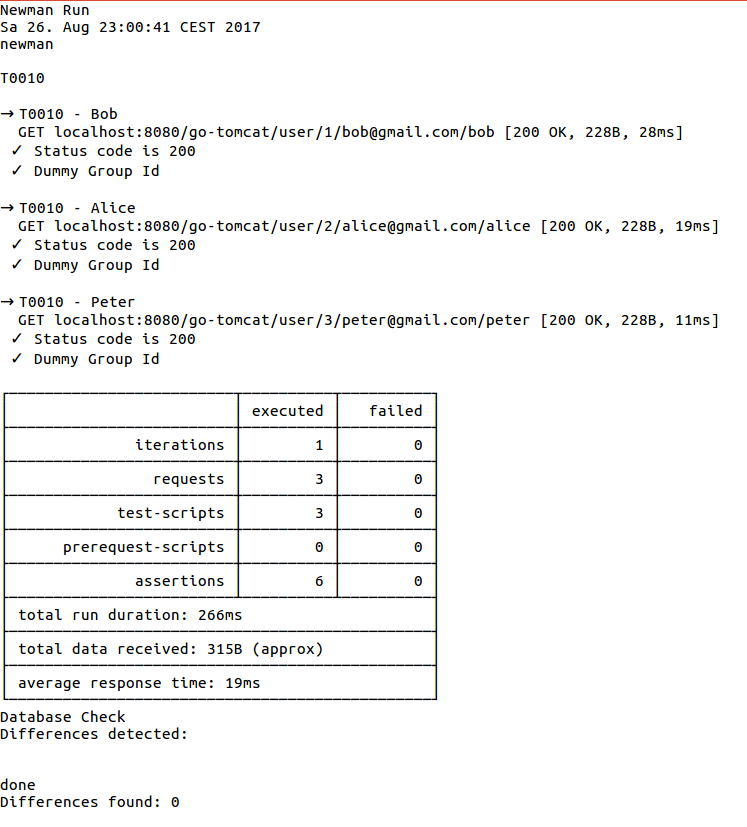
\includegraphics[width=1\textwidth]{result.png}
	\caption{Testbericht des Testfalls T0010 - alle Tests sind erfüllt}	
\end{figure}

\begin{figure}[H]
	\centering
	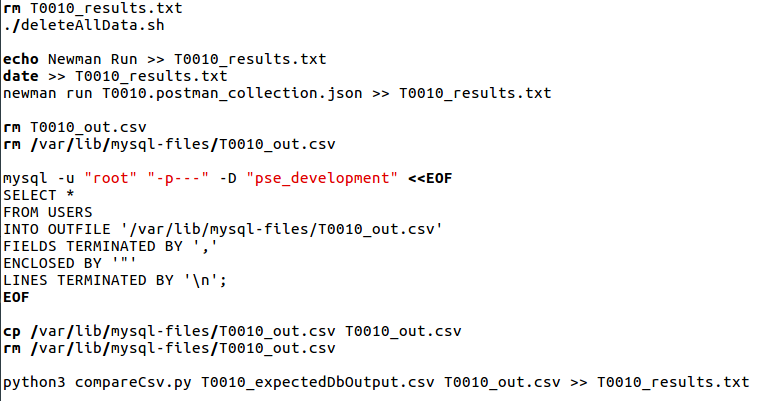
\includegraphics[width=1\textwidth]{test.png}
	\caption{Shell-Skript für den Testfall T0010 aus dem Pflichtenheft}	
\end{figure}


\subsubsection{durchgeführte Tests}
\begin{enumerate}
	\item[\textbf{/T0010/}]
	\textit{Testfall des Pflichtenhefts: }Der Testfall des Pflichtenhefts beschreibt das erstmalige Einloggen mit einem Google-Account, und damit die Erstellung eines Benutzeraccounts.\\
	\textit{Anfangsbedingungen: }Die Datenbank enthält noch keine Daten.\\
	\textit{Umsetzung auf die Serveranwendung: }Der Testfall entspricht dem Aufruf der Methode getData() auf dem Server über die Rest-API, wenn der aufgerufene Benutzeraccount noch nicht in der Datenbank existiert. Es werden drei API-Calls ausgeführt für drei verschiedende Benutzer.\\
	\textit{Erwartetes Ergebnis: } Der Respose-Body jedes API-Calls besteht aus einer Liste, die eine Dummy-Gruppe mit der Gruppen-ID 1 enthält, da keiner der Benutzer Mitglied in einer Gruppe ist. Nach der Ausführung der API-Calls sind die Benutzer mit den entsprechenden Daten in der Datenbank gespeichert.
	
	\item[\textbf{/T0040/}]
	\textit{Testfall des Pflichtenhefts: }Ein Benutzer loggt sich in seinem (existierenden) Benutzeraccount ein.\\
	\textit{Anfangsbedingungen: }Es befinden sich bereits Daten in der Datenbank (3 Benutzer, 1 Gruppe mit 2 Mitgliedern und 1 Gruppenanfrage, 1 Go)\\
	\textit{Umsetzung auf der Serveranwendung: }Der Tesetfall entspricht dem Aufruf der Methode \textit{getData()} über die Rest-API, wenn der aufgerufene Benutzeraccount bereits existiert. Es wird ein API-Call je angelegtem Benutzer durchgeführt.\\
	\textit{Erwartetes Ergebnis: }Der Response-Body jedes API-Calls gibt die Struktur der in den Anfangsbedingungen festgelegten Daten wieder. Die Responses sind identisch, da jeder Benutzer mit den gleichen Gruppen assoziiert ist. Es wird keine Manipulation der Daten auf der Datenbank vorgenommen.
	
	\item[\textbf{/T0050/}]
	\textit{Testfall des Pflichtenhefts: }Ein Benutzer löscht seinen Benutzeraccount\\
	\textit{Anfangsbedingungen: }Der Benutzer ist mit einem gültigen Account in der Datenbank gespeichert.\\
	\textit{Umsetzung auf der Serveranwendung: }Die Methode deleteUser() wird aufgerufen. Die Daten des Benutzers, sowie alle Gruppen und Gos, die ihm gehören werden gelöscht.\\
	\textit{Erwartetes Ergebnis: }Der Testfall-Benutzer ist Adminsitrator einer Gruppe. Es wird erwartet, dass die Gruppe, alle Gruppemmitglieder der Members-Tabelle, alle Requests der Requests-Tabelle, sowie der Eintrag des Benutzers in der Users-Tabelle gelöscht werden.
	
	\item[\textbf{/T0060/}]
	\textit{Testfall des Pflichtenhefts: }Ein Benutzer erstellt eine neue Gruppe.\\
	\textit{Anfangsbedingungen:}Der Benutzer ist mit einem gültigen Account in der Datenbank gespeichert.\\
	\textit{Umsetzung auf der Serveranwendung: }Die Methode createGroup() wird aufgerufen. Im request-Body befindet sich ein gültiger JSON-String, der ein Group-Objekt repräsentiert.\\
	\textit{Erwartetes Ergebnis: }Der Datenbank wird ein Tupel in der Group-Tabelle hinzugefügt, das dem übergebenen JSON-String entspricht. Darüber hinaus werden entsprechende Einträge in der Members- und Admins-Tabelle hinzugefügt. Der Response-Body enthält die ID unter der die Gruppe in der DB gespeichert ist.
	
	\item[\textbf{/T0070/}]
	\textit{Testfall des Pflichtenhefts: }Der Name einer Gruppe wird verändert\\
	\textit{Anfangsbedingungen:}Eine Gruppe ist in der Datenbank gespeichert.\\
	\textit{Umsetzung auf der Serveranwendung: }Aufruf der Methode editGroup(). Der Request-Body, enthält ein JSON-String, der dem geänderten Group-Objekt entspricht. Dabei sind nur die Attribute ID (zur Identifizierung der Gruppe in der DB), Name und Description relevant. Andere Attribute können auf diese Weise nicht geändert werden. Es wird ein API-Call ausgeführt, der den Namen der Gruppe ändert.\\
	\textit{Erwartetes Ergebnis: }Der neue Name der Gruppe ist in der Datenbank gespeichert.
	
	\item[\textbf{/T0090/}]
	\textit{Testfall des Pflichtenhefts: }Der Gruppenadministrator füt ein neues Mitglied hinzu, d.h. er verschickt eine Gruppenanfrage.\\
	\textit{Anfangsbedingungen:}Eine Gruppe ist in der Datenbank gespeichert und es existieren Benutzer, die nicht mit der Gruppe assoziiert sind.\\
	\textit{Umsetzung auf der Serveranwendung: }Aufruf der Methode inviteMember() und Übergabe der Email-Adresse des zu hinzufügenden Benutzers. Es werden 2 API-Calls ausgeführt, um 2 Gruppeneinladungen zu verschicken.\\
	\textit{Erwartetes Ergebnis: }Es werden der Tabelle Requests 2 Tupel hinzugefügt, mit jeweils der ID der Gruppe und der ID des eingeladenen Benutzers.
	
	\item[\textbf{/T0100/}]
	\textit{Testfall des Pflichtenhefts: }Eine zuvor verschickte Gruppenanfrage wird bestätigt.\\
	\textit{Anfangsbedingungen:}Es existiert eine Gruppe in der Datenbank und ein Eintrag in der Requests-Tabelle für diese Gruppe und den bestätigenden Benutzer.\\
	\textit{Umsetzung auf der Serveranwendung: }Aufruf der Methode acceptRequest().\\
	\textit{Erwartetes Ergebnis: }Der Eintrag der Requests-Tabelle wird entfernt und in die Members-Tabelle eingefügt.
	
	\item[\textbf{/T0110/}]
	\textit{Testfall des Pflichtenhefts: }Eine zuvor verschickte Gruppenanfrage wird abgelehnt.\\
	\textit{Anfangsbedingungen:}Es existiert eine Gruppe in der Datenbank und ein Eintrag in der Requests-Tabelle für diese Gruppe und den bestätigenden Benutzer.\\
	\textit{Umsetzung auf der Serveranwendung: }Aufruf der Methode denyRequest().\\
	\textit{Erwartetes Ergebnis: }Der Eintrag der Requests-Tabelle wird entfernt.
	
	\item[\textbf{/T0130/}] \label{T130} 
	\textit{Testfall des Pflichtenhefts: }siehe \ref{130} /T0130/\\
	\textit{Anfangsbedingungen:}Es existiert eine Gruppe in der Datenbank\\
	\textit{Umsetzung auf der Serveranwendung: }Aufruf der Methode deleteGroup().\\
	\textit{Erwartetes Ergebnis: }Die Gruppe, sowie alle Daten, die mit der Gruppe assoziiert (Gos, Members, Admins, Requests), sind werden gelöscht.
	
	\item[\textbf{/T0160/}]
	\textit{Testfall des Pflichtenhefts: }Ein Mitglied einer Gruppe wird entfernt.\\
	\textit{Anfangsbedingungen: }Es existiert eine Gruppe in der Datenbank unnd der zu entfernende Benutzer ist nicht der Administrator der Gruppe.\\
	\textit{Umsetzung auf der Serveranwendung: }Aufruf der Methode removeMember().\\
	\textit{Erwartetes Ergebnis: }Der Eintrag in der Member-Tabelle wird entfernt. Zusätzlich werden alle Gos des entfernten Benutzers und die damit assoziierten Daten (Going Users, Not Going Users, Gone Users) gelöscht.
	
	\item[\textbf{/T0170/}] wird von Testfall \ref{T130} /T0130/ abgedeckt
	
	\item[\textbf{/T0180/}]
	\textit{Testfall des Pflichtenhefts: }Erstellen eines GOs\\
	\textit{Anfangsbedingungen:}Es exisitert eine Gruppe in der Datenbank\\
	\textit{Umsetzung auf der Serveranwendung: }Aufruf der Methode createGo(). Als Argument wird das im Request-Body als JSON-String übertragene GO-Objekt übergeben.\\
	\textit{Erwartetes Ergebnis: }Es wird ein Eintrag in der Tabelle GOs erstellt, die dem übergebenen GO-Objekt entspricht. Für den GO-Verantwortlichen wird ein Eintrag in der Tabelle Going-Users erstellt. Für jedes weitere Gruppenmitglied wird ein Eintrag in der Tabelle Not-Going-Users erstellt.
	
	\item[\textbf{/T0200/}]
	\textit{Testfall des Pflichtenhefts: }Änderung des Teilnahmestatus (im Pflichtenheft von Abgelehnt auf Bestätigt).\\
	\textit{Anfangsbedingungen:}Es existiert ein Go in der Datenbank.\\
	\textit{Umsetzung auf der Serveranwendung: }Aufruf der Methode changeStatus(). Der betroffenen Benutzer, sowie der neue Status, werden im Request-Body übergeben. Es werden 3 API-Calls ausgeführt mit jeweils einem Statuswechsel von Going zu Gone, Gone zu Going und Not Going zu Going.\\
	\textit{Erwartetes Ergebnis: }Der alte Eintrag des Benutzers in den Status-Tabellen (Going-Users, Not-Going-Users, Gone-Users) wird entfernt und ein neuer, entspechend dem neuen Status eingefügt.
	
	\item[\textbf{/T0250/}]
	\textit{Testfall des Pflichtenhefts: }Ein GO wird beendet.\\
	\textit{Anfangsbedingungen:}Es existiert ein GO in der Datenbank.\\
	\textit{Umsetzung auf der Serveranwendung: }Die Beendigung eines GOs ist gleichzusetzen mit dem Löschen eines Gos. Es wird die Methode deleteGo() aufgerufen.\\
	\textit{Erwartetes Ergebnis: }In der Datenbank wird das entsprechende GO gelöscht, sowie alle damit assoziierten Informationen (Einträge in den Status-Tabellen Going-Users, Not-Going-Users und Gone-Users).
	
	\item[\textbf{/T0260/}]
	\textit{Testfall des Pflichtenhefts: }Die Daten eines GOs werden geändert.\\
	\textit{Anfangsbedingungen:}Es exisitert ein GO in der Datenbank.\\
	\textit{Umsetzung auf der Serveranwendung: }Aufruf der Methode editGo(). Die geänderte Gruppe wird dabei als JSON-String im Request-Body übertragen. es wird ein API-Call durchgeführt, der den Namen des GOs ändert.\\
	\textit{Erwartetes Ergebnis: }Der geänderte Name des GOs wird in der Datenbank gespeichert.
	
	\item[\textbf{/T0360/}]
	\textit{Testfall des Pflichtenhefts: }siehe \ref{360} /T0360/\\
	\textit{Anfangsbedingungen:} Es existiert ein Benutzeraccount in der Datenbank.\\
	\textit{Umsetzung auf der Serveranwendung: }Aufruf der Methode registerDevice(). Es werden drei API-Calls ausgeführt, um allen drei existierenden Benutzern in der Datenbank eine InstanceId zuzuweisen.\\
	\textit{Erwartetes Ergebnis: }Die InstanceId wird jeweils in dem Tupel des Benutzers in der Datenbank gespeichert.
	
\end{enumerate}

\newpage

\section{Hallway Usability Test}

\newpage

\section{Bugs}

\begin{enumerate}[label={\textbf{/B\protect\threedigits{\theenumi}0/}}, leftmargin=*]
\item \textbf{FCM-Message nicht an Client gesendet nach dem Löschen einer Gruppe}
	\begin{itemize}
		\item[Symptom]
		Nachdem ein User eine Gruppe gelöscht hat, wird keine Message an die anderen Gruppenmitglieder gesendet, um sie über die Löschung der Gruppe zu informieren. Dies führt zu inkonsistenten Daten auf den verschiedenen Endsystemen.
		\item[Ursache]
		Der GroupRemovedObserver, der für die Versendung der richtigen Message zuständig ist, versucht die zu informierenden Gruppenmitglieder aus der Datenbank zu finden, nachdem die Gruppe in der Datenbank bereits gelöscht wurde. Dies löst eine NullPointerException aus, da auf nicht (mehr) existierende Objekte zugegriffen wird, und das Versenden der Messages wird abgebrochen.
		\item[Behebung]
		Die Receiver-Liste, die der Observer zur Adressierung der Gruppenmitglieder verwendet wird erstellt, \textbf{bevor} die Gruppe aus der Datenbank gelöscht wird. So muss nach der Löschung kein Datenbankzugriff mehr stattfinden, um die Messages korrekt zu senden.
	\end{itemize}

\item \textbf{StackOverflow bei automatisierter JSON Konvertierung}
	\begin{itemize}
		\item[Symptom]
		Das System stürzt ab, sobald ein JSON-String einer Entity-Klasse erstellt werden soll.
		\item[Ursache]
		Durch zyklische Abhängigkeiten (Gruppen entalten GOs, GOs enthalten ein Gruppe) kommt es bei der Konvertierung zu einem StackOverflow.
		\item[Behebung]
		Bevor Entities konvertiert werden, werden die durch die passende \textit{makeJsonable()}-Methode angepasst, sodass sie sicher konvertiert werden können, ohne dass es zu einem StackOVerflow kommt und ohne, dass wichtige Informationen verloren gehen.
	\end{itemize}

\item \textbf{Rückgabe von Null-Werten bei Suche eines Users anhand der Email-Adresse}
	\begin{itemize}
		\item[Symptom] In Anwendungsfällen, in denen ein Benutzer anhand seiner E-Mail-Adresse in der Datenbank gefunden wurde, wird \textit{null} zurückgegeben, wodurch die weitere Abarbeitung des Anwendungsfalls nicht möglich ist.
		\item[Ursache] Die URI, mit der die Anfrage an den Server gestellt wird endet mit der E-Mail-Adresse des Benutzers, woraufhin das '.com' am Ende der E-Mail-Adresse abgeschnitten wird. Durch die fehlende TLD, kann die richtige E-Mail-Adresse in der Datebank nicht identifiziert werden.
		\item[Behebung] Bevor die Anfrage an die Datenbank weitergeleitet wird, wird die Endung '.com' an die gesuchte E-Mail-Adresse angefügt. Da es sich bei den Adressen stets um gmail-Accounts handelt, muss nicht zwischen mehreren TLDs unterschieden werden.
	\end{itemize}
	
\item \textbf{Vertauschung der angezeigten Gruppe, bei Änderung des Gruppennamens}
	\begin{itemize}
		\item[Symptom] Befindet sich ein Benutzer in der Detailansicht einer Gruppe und ändert den Namen derselben, wird nach Ausführung der Aktion die Detailansicht einer anderen Gruppe angezeigt.
		\item[Ursache] Die Gruppen sind alphabetisch gespeichert, um sie in dieser Reihenfolge anzeigen zu können. Ändert sich ein Gruppenname, ändert sich auch die Reihenfolge in der die Gruppen in der ArrayList im ViewModel gespeichert sind. Da die aktuell angezeigte Gruppe durch ihren Index in der ArrayListe des ViewModels identifiziert wird, wird nach einer Änderung dieser Liste fälschlicherweise die Gruppe angezeigt, die nun diesen Index trägt.
		\item[Behebung] %TODO bitte ergänzen, @Arsenii ich glaube du hast das gemacht
	\end{itemize}

\end{enumerate}

\newpage

\section*{Anhang}

\subsection*{A. Testberichte zu Abschnitt \ref{ServerIT}}


\end{document}
\grid
